%*******************************************************************************
%*********************************** Third Chapter *****************************
%*******************************************************************************


\chapter{Criptografia}

O surgimento da criptografia (do grego:Kryptós,oculto + graph, r.de graphein, escrever) remota a milhares de anos, sendo uma das técnicas mais antigas na transmissão de informação de forma secreta. No ano 400 a.C., os Espartanos conceberam um método intrigante: eles gravavam mensagens em uma tira de couro enrolada em um bastão. Ao desenrolar a tira do bastão, a mensagem era cifrada, requerendo que fosse enrolada novamente em um bastão de diâmetro similar para decifrá-la~\cite{Quaresma2009a}.

Um sistema criptográfico é então um conjunto de procedimentos que possibilitam tornar uma mensagem ilegível para qualquer pessoa que não seja o destinatário autorizado, garantindo que somente o destinatário legítimo possa decodificá-la e acessar o conteúdo original~\cite{Quaresma2009a}.

Portanto, a criptografia tem os seguintes objetivos:
\begin{description}
    \item[Confidencialidade] Manter o conteúdo da informação confidencial para todos exceto o destinatário;
    \item[Integridade da informação] Certificar-se de que não há adulteração da informação por partes não autorizadas;
    \item[Autenticação] {\ }
    \begin{itemize}
        \item das entidades que comunicam entre si;
        \item da informação (origem, conteúdo, data de envio,$\dots$)
    \end{itemize}
    \item[Não repudiação] o criador da informação não pode negar a autoria.
\end{description}

\section{Sistemas Criptográficos Simétricos}
\label{sec:SistemasCriptograficosSimetricos}

Os primeiros sistemas criptográficos desenvolvidos foram baseados na criptografia simétrica, conhecida como sistemas de chave secreta. Esses sistemas utilizam uma única chave para cifrar e decifrar informações, onde os processos de encriptação e desencriptação são idênticos.

Mas, esses sistemas enfrentam dois problemas que limitam a sua eficácia na proteção das informações:

A chave de cifração deve ser compartilhada por todos os elementos da organização ``amiga'' e, ao mesmo tempo, deve ser mantida em segredo absoluto de organizações consideradas como adversárias. Quanto mais complexa for a estrutura da organização ``amiga'', mais complicado será garantir esta condição~\cite{Quaresma2009a}.

\section{Sistemas Criptográficos Assimétricos}
\label{sec:SistemasCriptograficosAssimetricos}
Aparecem então os sistemas de criptografia assimétrica, ou de chave pública. Nestes sistemas, a cifragem utiliza uma chave diferente, conhecida como chave privada.

Este tipo de sistema resolve os dois problemas mencionados anteriormente:


Os algoritmos desenvolvidos são significativamente mais complexos para serem quebrados em comparação com os sistemas anteriores.

\begin{itemize}
    \item[+] A chave privada é conhecida por apenas uma única entidade, o destinatário da mensagem. Manter essa chave secreta torna-se assim consideravelmente mais simples;
    \item[-] os algoritmos desenvolvidos são menos eficientes do que as atuais cifras do tipo simétrico.
\end{itemize}

Para avaliar as ferramentas criptográficas utilizam-se os seguintes parâmetros:
\begin{description}
   \item[Nível de Segurança] número de operações solicitadas pelo melhor método conceituado para quebrar o código;
   \item[Funcionalidade]  quais são as primitivas mais eficientes para uma dada finalidade;
   \item[Método de Operações] o procedimento de cada primitiva depende da maneira como são aplicadas e de quais os valores que lhe são dados;
   \item[Performance] as ferramentas têm de ser eficientes em termos de tempo e espaço;
   \item[Facilidade de Implementação] implementar uma dada ferramenta num dado sistema operacional de forma simples.
\end{description}

Para criar um esquema de encriptação vamos precisar selecionar:

\begin{itemize}
    \item um alfabeto(finito) definição;
    \item um espaço de mensagens
    \item um espaço de chaves;
    \item um conjunto de transformações de encriptação;
    \item um correspondente conjunto de transformações de desencriptação
\end{itemize}

Para tal vão ser introduzidas , formalmente, as seguintes definições:

\begin{definicao}[Alfabeto de Definição]$\mathcal{A}$ denota de um conjunto finito de símbolos designado por alfabeto de definição.
\end{definicao}

\begin{definicao}[Espaço das Mensagens] $\mathcal{M}$ denota um conjunto designado por espaço das mensagens. $\mathcal{M}=\mathcal{A^*}$ consiste de sequências de elementos de um alfabeto de definição. Um elemento de $\mathcal{M}=\mathcal{A^*}$  é designado por mensagem de texto claro (não cifrado).
\end{definicao}

\begin{definicao}[Espaço das Mensagens Cifradas]
$\mathcal{C}$ denota um conjunto designado por espaço das mensagens cifradas. $\mathcal{C}$ consiste de sequências de elementos de um dado alfabeto de definição, o qual pode diferir do usado em $\mathcal{M}$. Um elemento de $\mathcal{C}$ é designado por texto cifrado.
\end{definicao}

\begin{definicao}[Definição das chave] $\mathcal{K}$ denota um conjunto designado por espaço das chaves. Um elemento de $\mathcal{K}$ é designado por chave.
\end{definicao}

\begin{definicao}[Função de Encriptação] Cada elemento $e \in \mathcal{K}$ determina, de forma única, uma bijeção de $\mathcal{M}$ para $\mathcal{C}$, designada por $\mathcal{E}_e$ é designada por função de encriptação, ou transformação de encriptação.
\end{definicao}

\begin{definicao}[Função de Desencriptação] para cada $d \in \mathcal{K}$, $\mathcal{D}_d$ denota a bijeção de $\mathcal{C}$ para $\mathcal{M}$. $\mathcal{D}_d$ é designada por função de desencriptação, ou transformações de desencriptação.
\end{definicao} As funções $\mathcal{D}_d e \mathcal{E}$ devem ser tais que se verifica:

$$\mathcal{D}_d(E_e(m))=m$$

\begin{definicao} [Encriptaçao] o processo de aplicar a transformação $E_e$ a mensagem $m \in M$ é usualmente designado por encriptar $m$, ou a encriptação de $m$, onde $M$ é o espaço das mensagens.
\end{definicao}

\begin{definicao}[Desencriptação]
O processo de aplicar a transformação $D_d$ ao texto cifrado $c \in C$ é usualmente designado por desencriptar $c$, ou a desencriptação de $c$, onde $C$ é o espaço das mensagens cifradas.
\end{definicao}

\begin{definicao} [Par de Chaves] As chaves $e$ e $d$ na definição anterior são designadas por par de chaves, e usualmente denotadas por $(e,d)$. Note-se que as chaves podem ser iguais.
\end{definicao}

\begin{definicao}[Esquema de Encriptação---Cifra] Um esquema de encriptação consiste de um conjunto $\{E_e : e \in K\}$ de transformações de encriptação e um conjunto correspondente $\{D_d:d \in K\}$ de transformações de desencriptação com a propriedade de que para todo o $e \in K$ existe uma chave única $d \in K$ tal  que $D_d=E_d^{-1}$, isto é, $D_d(E_e(m))=m$ para todo o $m \in M$, onde $K$ é o espaço de chaves K, $\{E_e :e \in K\}$ um conjunto de transformações de encriptação e $\{D_d :d \in K\}$ de transformações de desencriptação.
\end{definicao}

\begin{figure}[h]
    \centering
    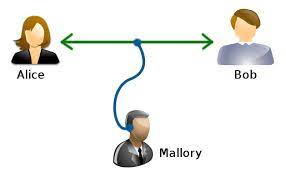
\includegraphics[scale=0.5]{Figs/bobalice.jpg}
    \caption{Bob e Alice}
    \label{fig:bobalice}
\end{figure}
Exemplificando, tem-se as seguintes etapas na utilização de uma cifra:
\begin{description}
    \item[Utilização de uma cifra de chaves simétricas] {\ }
    \begin{enumerate}
        \item Alice e Bob escolhem (secretamente) um par de chaves;
        \item Bob decide enviar uma mensagem, $m \in \mathcal{M}$, a Alice. Calcula $c=E_e(m)$ e envia o texto resultante;
        \item Ao receber a mensagem a Alice calcula $D_d(c)=m$ recuperando deste modo a mensagem original.
    \end{enumerate}
    \item[Utilização de uma cifra de chaves assimétricas] {\ }
    \begin{enumerate}
        \item O Bob escolhe um par de chaves: torna pública a chave de encriptação $e$, mantém secreta a chave de desencriptação $d$.
        \item A alice decide enviar uma mensagem, $m \in \mathcal{M}$, ao Bob. Obtém a chave pública do Bob $e$ e calcula $c=E_e(m)$. Depois envia o texto resultante.
        \item Ao receber a mensagem o Bob calcula $D_d(c)=m$ recuperando deste modo a mensagem original.
    \end{enumerate}
\end{description}

Assim, Bob e Alice conseguem comunicar secretamente, sem conceder ao Mallory acesso ao conteúdo da conversa.

Naturalmente todo o código têm duas etapas: uma para codificar a mensagem e outra para decodificar a mensagem. Mas para decifrar uma mensagem, isto é, ler um mensagem codificada sem ser o verdadeiro destinatário dela é preciso ``quebrar'' o código. Portanto é necessário introduzir a seguinte definição:

\begin{definicao}[Criptoanálise] É o estudo dos procedimentos necessários para tentar comprometer as técnicas criptográficas, e mais genericamente, os serviços de segurança da informação.
\end{definicao}

\begin{definicao}[Cifra (parcialmente) Quebrada] É o ataque sistemático a uma cifra com a finalidade principal de obter texto claro a partir de texto cifrado. Em caso de sucesso, diz-se que a cifra for parcialmente quebrada.
\end{definicao}

\begin{definicao}[Cifra (formalmente) Quebrada] Tem por objetivo obter a chave privada de uma entidade, nesse caso a cifra é completamente e formalmente quebrada.
\end{definicao}

Relativamente as classes de ataques aos esquemas de encriptação, tem-se as seguintes definições:

\begin{definicao}[Ataque Passivo] É um ataque em que o adversário apenas monitoriza o canal de comunicação. Um atacante passivo apenas ameaça a confidencialidade da informação.
\end{definicao}

\begin{definicao}
[Ataque Ativo] É um ataque em que o adversário tenta apagar, acrescentar, ou de alguma forma modificar a informação. Um atacante ativo ameaça a integridade da informação assim como a sua confidencialidade.
\end{definicao}

Em relação ao tipo de ataque, tem-se as seguintes definições:

\begin{definicao}[Ataque de texto cifrado] neste tipo de ataque o criptoanalista tenta deduzir a chave de decifração ou o texto claro por observação unicamente do texto cifrado. Uma cifra que seja vulnerável a este tipo de ataque considera-se completamente inseguro.
\end{definicao}

\begin{definicao}[Ataque de texto claro conhecido] É um ataque aonde o criptoánlista consegue obter um excerto de um texto claro com base num seu corresponde teste cifrado.
\end{definicao}

\begin{definicao} [Ataque de texto claro escolhido]É um ataque aonde o adversário escolhe o texto em claro obtendo de seguida o corresponde texto cifrado. Toda a informação daí deduzida é posteriormente usada em outros textos cifrados.
\end{definicao}

\begin{definicao} [Ataque de de força bruta] É um ataque por procura exaustiva no espaço das chaves. Uma cifra sujeita a este tipo de ataque é designado por cifra fraca.
\end{definicao}


Por exemplo, suponhamos que o Mallory, extremamente perspicaz, conseguiu encontrar uma forma de comprometer os métodos de encriptação e desencriptação utilizados pelo Bob e a Alice. Primeiramente, efetuou a monitorização das conversas trocadas pelo Bob e Alice tendo conseguido chegar ao texto cifrado a partir de um certo texto original que conseguiu reunir antes do Bob enviar para a Alice. 
Apercebendo-se do quanto o conteúdo da informação era preciosa, Mallory quis impedir Alice de ter acesso ao resto do informação.
Para isso encontrou a chave certa testando todas as chaves disponíveis. E com isso conseguiu,facilmente, decifrar o conteúdo dos textos cifrados do Bob e passou a enviar falsas correspondências, em nome do Bob, a alice.
\begin{figure}[h]
    \centering
    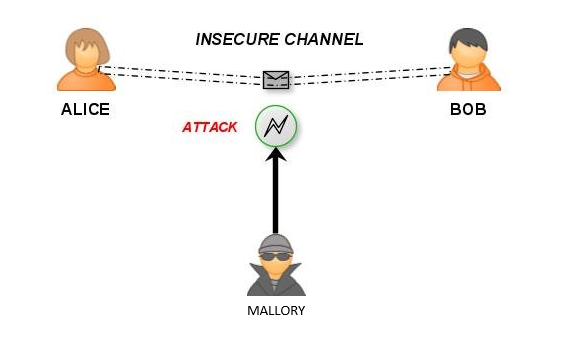
\includegraphics[scale=0.5]{Figs/mallory.PNG}
    \caption{Bob, Alice e Mallory}
    \label{fig:bobalice}
\end{figure}

Observação: Num sistema de chave pública é preciso saber a chave pública do destinatário de modo a encriptar uma mensagem a ele destinada. Apenas o destinatário é capaz de decifrar a mensagem.

Nota: Cada entidade tem um par (chave pública, chave privada). De forma a evitar ataques as chaves públicas disponibilizadas pelas entidades, tais como, a substituição da chave pública (este tipo de ataque é designado por personificação) foi criado um repositório de chaves que é capaz de garantir a manutenção das chaves~\cite{Quaresma2009a}.

